\chapter{Methodology}
\label{sec:methodology}

This chapter explains how things were done within the duration of the whole project. Section \ref{sec:project_overview} gives an overview of the whole project and its goals. Section \ref{sec:task_division} explains how the work was divided between all parties involved in the development of this project. Section \ref{sec:game_gathering} shows how and which games were selected for both parts of this work. Section \ref{sec:packaging} clarifies how the packaging template was created and its main parts. Section \ref{sec:platform_development} illustrates how the platform was developed. Section \ref{sec:tools} references the tools that were used to create and test everything the project has aimed to create.

\section{Project Overview}
\label{sec:project_overview}

The project had the main goal of creating a platform for all the games developed in the university's courses related to games. The games that will be available must have all their assets and required libraries in packages that run on some GNU/Linux, Windows and macOS systems.

In order to achieve this goal, the games developed in this \textit{campus} of the University were cataloged and cloned into a main GitHub organization \footnotemark (whenever possible). A template system was created to package the files for each one of the contemplated Operating Systems.

The platform itself was developed while all the other activities took place, during the first half of this work. Some games were chosen to test the template, but its main use will be during the new development cycle inside the game courses.

\footnotetext{\href{https://github.com/unbgames}{https://github.com/unbgames/}}

\section{Task Division}
\label{sec:task_division}

This project was totally collaborative, it depended and relied on different classes and courses. Because of that, during the first half of it, the work was divided among students and teachers, as illustrated in Figure \ref{fig:task_division}.

\begin{figure}[h!]
\centering
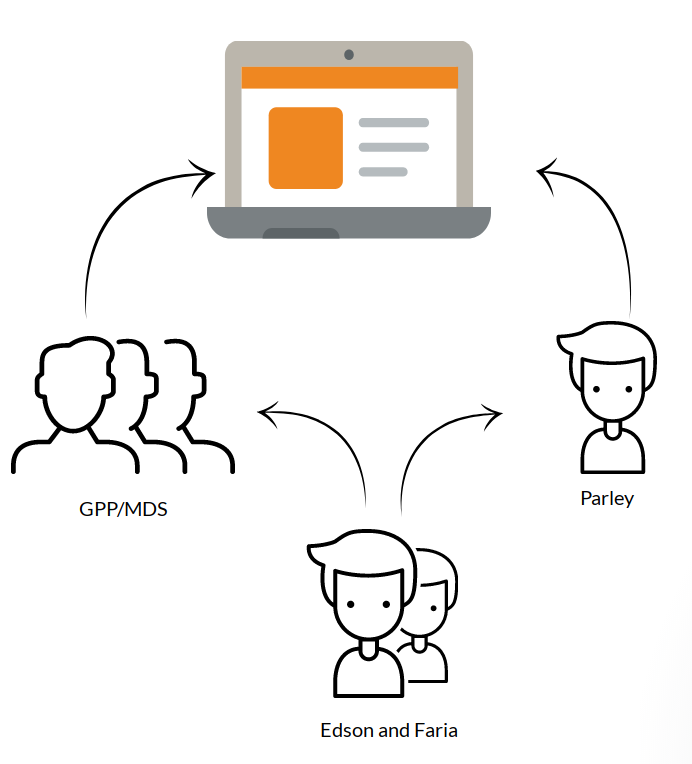
\includegraphics[width=200px,height=\textheight,keepaspectratio]{task_division}
\caption{Task Division}
\label{fig:task_division}
\end{figure}

Professor Edson and Mr. Faria were responsible for first cataloging the existing games. They remained as helpers in the packaging system and main stakeholders for the team that developed the website.

The team \textit{Plataforma de Jogos UnB} from the courses \textit{M\'etodos de Desenvolvimento de Software} (Software Development Methods) and \textit{Gest\~ao de Portfolios e Projetos} (Management of Portfolios and Projects) was in charge of creating the first version of the actual website with some of the features desired. The names of all the members are in the Appendix \ref{sec:members_gpp_mds}.

Before the second half of the project, professor Edson developed the packaging template. During this term, my responsibility was to test this template in a few selected games and to evolve and maintain it, as well as to maintain and add some features to the platform developed in the previous semester. Professor Edson and Mr. Faria were code reviewers and helpers in the system.


\section{Game Gathering}
\label{sec:game_gathering}

The games selected for the first part of the project were the ones developed in this department, \textit{Faculdade UnB Gama} that is the Gama \textit{campus} of the University since the course \textit{Introdu\c{c}\~ao aos Jogos Eletr\^onicos} (Introduction to Electronic Games) has been created here in the first semester of 2012. Professor Ricardo Jacobi was the first to teach the course, but it wasn't possible to contact him or get the games developed in that term. Professor Edson taught the course after that, until 2016. It has been assumed by Mr. Matheus Faria, since the beginning of this year (2017).

Because this work was being mostly held at FGA, and all the games developed here are compiled and run on Linux distributions, these were selected as first games for the platform. Another reason for this choice is the proximity with the students who created those games.

Professor Edson and Mr. Faria first contacted the students and asked them to post their codes to GitHub. They cloned them into the \texttt{fgagamedev}\footnote{ \href{https://github.com/fgagamedev}{https://github.com/fgagamedev/} } GitHub organization.

After that, I was responsible for checking the status of the games, gathering information such as which of them compiled, which SDL version they used, which ones had licenses. Table \ref{tab:first_games} shows these initial results.


\begin{table}[h!]
\centering
\caption{Initial status of the selected games}
\label{tab:first_games}
\rowcolors{2}{gray!30}{white}
\begin{tabular}{lccccc}
\toprule
\textbf{Name} & \textbf{Source?} & \textbf{License?} & \textbf{SDL} & \textbf{Compiles?} & \textbf{Year}\\
\midrule
Deadly Wish & y & n & 2 & n & 2016 \\
Strife of Mythology & y & n & 2 & y & 2016 \\
Travelling Will & y & n & 2 & y & 2016 \\
7 Keys & y & MIT & 2 & n & 2015 \\
Babel & y & GPL 2 & 2 & y & 2015 \\
Terracota & y & MIT & 2 & n & 2015 \\
Dauphine & y & n & 2 & n & 2014 \\
Imagina na Copa & y & n & 2 & y & 2014 \\
Kays Against the World & y & n & 2 & y & 2014 \\
Ankhnowledge & y & GPL 2 & 1 & y & 2013 \\
The Last World War & n & - & - & - & 2013 \\
Post War & y & n & 1 & y & 2013 \\
War of the nets & y & GPL 2 & 2 & y & 2013 \\
Jack the Janitor & y & GPL 3 & 1 & y & 2013 \\
Drawing Attack & n & - & - & - & 2012 \\
Earth Attacks & n & - & - & - & 2012 \\
Emperor vs Aliens & y & n & 1 & y & 2012 \\
Ninja Siege & y & GPL 2 & 1 & y & 2012 \\
Space monkeys & y & GPL 2 & 1 & n & 2012 \\
Tacape & n & - & - & - & 2012 \\
\bottomrule
\end{tabular}
\end{table}

Out of 20 games created in \textit{Introdu\c{c}\~ao aos Jogos Eletr\^onicos} while Professor Edson taught it, 4 didn't have a known repository and 8 didn't have a license that allowed us to change them at that time. Mr. Faria and I were responsible for finding unknown games and getting the missing licenses. As result of this task, \textit{The Last World War} was added and 5 other had licenses acquired as shown in Table \ref{tab:final_games}.

\begin{table}[h!]
\centering
\caption{Game status after contacting developers}
\label{tab:final_games}
\rowcolors{2}{gray!30}{white}
\begin{tabular}{lccc}
\toprule
\textbf{} & \multicolumn{1}{l}{\textbf{License}} & \multicolumn{1}{l}{\textbf{SDL}} & \multicolumn{1}{l}{\textbf{Compiles}} \\
\midrule
Deadly Wish & GPL 3 & 2 & n \\
Strife of Mythology & GPL 2 & 2 & y \\
Travelling Will & MIT & 2 & y \\
7 Keys & MIT & 2 & n \\
Babel & GPL 2 & 2 & y \\
Terracota & MIT & 2 & n \\
Dauphine & MIT & 2 & n \\
Imagina na Copa & MIT & 2 & y \\
Kays Against the World & n & 2 & y \\
Ankhnowledge & GPL 2 & 1 & y \\
The Last World War & n & 1 & y \\
Post War & MIT & 1 & y \\
War of the nets & GPL 2 & 2 & y \\
Jack the Janitor & GPL 3 & 1 & y \\
Emperor vs Aliens & n & 1 & y \\
Ninja Siege & GPL 2 & 1 & y \\
Space monkeys & GPL 2 & 1 & n \\
\bottomrule
\end{tabular}
\end{table}

In the second semester, to test the new packaging template, four games were selected. two out of those previously chosen, developed with SDL, and two new ones developed in the first semester of 2017, made with SDL2: \textit{Ankhnowledge}, \textit{Ninja-Siege}, \textit{Wenova}, and \textit{Mindscape}, respectively. These games were chosen because they already worked correctly without any need to change their source code.

Another decision was to separate the games in a different GitHub organization, to hold all the ones developed at the University, instead of just those from FGA. Matheus created the \texttt{unbgames} organization for this purpose and \texttt{fgagamedev} remained as an FGA specific organization, where the packaging template is maintained, for example.

\section{Packaging}
\label{sec:packaging}

The template for packaging was created by professor Edson is based on two main directives, modularisation and platform independence. The first one is related to dividing the directories by topic, meaning that each folder will be responsible for one thing and all the files inside of them should be related to that specific thing. The second directive, platform independence, is to make the development for multiple platforms easy. Each directory will have a division for each of the platforms.

To achieve the template modularisation, professor Edson decided to use a folder structure that would be easy to understand to anyone familiar with GNU/Linux FHS, with a few additions. Apart from the original directories in the repository, he added the folders \texttt{bin}, \texttt{dist}, \texttt{lib} and \texttt{scripts}. This structure is represented in Figure \ref{fig:folder_structure}

\begin{itemize}

\item \texttt{bin} has all needed libraries and the game executable.
\item \texttt{lib} All the third-party libraries should live here. The scripts to build the code are already set to look for libs inside this directory, being each subdirectory a dependency;
\item \texttt{dist} This contains the files needed to generate the packages for each platform;
\item \texttt{scripts} this is where the scripts to build, package and distribute the binaries for all the platforms will live. It also has a subdirectory called \texttt{utils} that holds some specific platform scripts, like generating each installer, or gather information about the host OS;
\end{itemize}

\begin{figure}[h!]
\centering
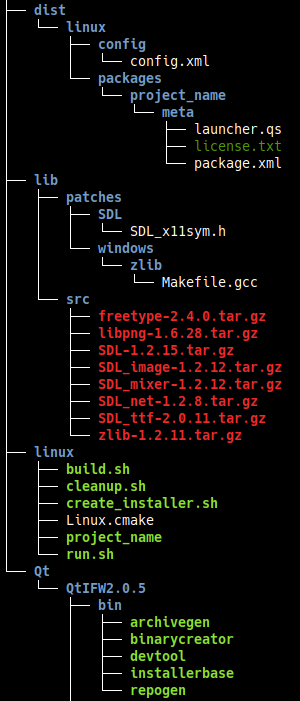
\includegraphics[scale=0.7]{folder_structure}
\caption{Folder tree}
\label{fig:folder_structure}
\end{figure}

The second directive was met by dividing some of the directories into platform limited directories, making the code that lives there accessible only when running on that individual platform. Any file outside the platform directory is considered generic and can be used for any Operating System. For example, when running on Windows, the compiler would only access generic files and Windows specific ones, like \texttt{dlls}. The same thing happens for macOS and GNU/Linux systems. This division is represented inside the \texttt{lib} directory in Figure \ref{fig:folder_structure_lib}.

\begin{figure}[h!]
\centering
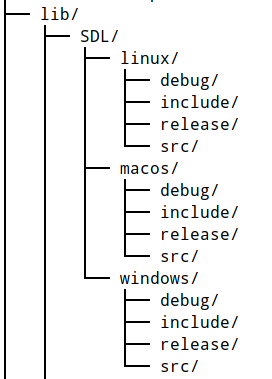
\includegraphics[scale=0.7]{folder_structure_lib}
\caption{Library division}
\label{fig:folder_structure_lib}
\end{figure}

As also seen in Figure \ref{fig:folder_structure_lib}, inside each platform folder (only for libraries) there is yet another division to make sure the template can generate different versions of the program for \texttt{debug} and \texttt{release}. The binaries that live on \texttt{release} are stripped of all debug symbols, resulting in smaller versions of those dependencies. Library headers go inside \texttt{include} and a compressed file with the source goes inside \texttt{src}.


The scripts kept in the \texttt{scripts} directory are the backbone of the template. Through them, it's possible to compile (creating a new executable with all the dependencies locally available), run and package a game. As long as the other files are placed correctly, the scripts work properly. There are four main and seven auxiliary scripts to accomplish these tasks, that are listed in Figure \ref{fig:folder_structure_scripts} and described below.

\begin{figure}[h!]
\centering
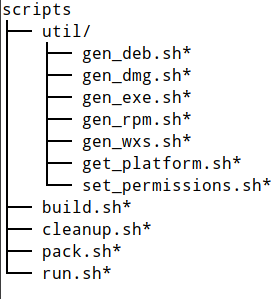
\includegraphics[scale=0.7]{folder_structure_scripts}
\caption{Scripts}
\label{fig:folder_structure_scripts}
\end{figure}

\begin{itemize}
    \item \texttt{build.sh} builds the executable, being possible to choose which is the desired version, \texttt{debug} and \texttt{release}. Calls the appropriate \texttt{Makefile}, depending on the version and platform;
    \item \texttt{cleanup.sh} clears the repository, removing files generated during build and packaging, like object files and installers;
    \item \texttt{pack.sh} builds the release version of the program (by calling \texttt{build.sh}) and generates the installer for the specific platform it's running on. It's important to notice that it's not possible to generate a package for a different platform from the same host system. This means that, for example, to generate Windows packages, this script must be called from within Windows and not from a Linux machine;
    \item \texttt{run.sh} runs the generated executable, setting the correct environment variables and pointing to where the local libs are. Attempting to run the program without this script may lead to errors;
    \item \texttt{util/get\_platform.sh} checks and returns the current platform;
    \item \texttt{util/set\_permissions.sh} sets files to 644\footnote{644 - File owner has read and write permissions, while group and all users have only read access.} permission and folders to 755\footnotemark inside a given directory;
    \item \texttt{util/gen\_deb.sh} generates a \texttt{.deb} file to be installed in Debian-based systems;
    \item \texttt{util/gen\_rpm.sh} generates an \texttt{.rpm} file to be installed in Red Hat based systems;
    \item \texttt{util/gen\_exe.sh} generates the \texttt{.exe} and \texttt{.msi} to be installed on Windows systems;
    \item \texttt{util/gen\_wxs.sh} This is called from \texttt{gen\_exe} to create a \texttt{.wxs} file, that will be used to create the Windows intaller.
    \item \texttt{util/gen\_dng.sh} creates the \texttt{.dmg} file for macOS.
\end{itemize}


All the scripts described in this section must be executed from the root folder of the repository. All paths inside the scripts are relative to that directory and running them anyplace else may cause unwanted errors.

\footnotetext{755 - File owner has read, write and execute permissions, while group and all users have read and execute permissions.}

\section{Platform Development}
\label{sec:platform_development}

The first version of the platform was developed using mixed development methods. During the first half of the semester, the Rational Unified Process and the PMBOK were used. For the next part, Scrum and XP were chosen. This choice of development framework is because of how the courses are divided.

Throughout the RUP part of the development, the team created several documents to aid the development cycle, such as vision, architecture document, class diagram, use case diagram, use case specification, test case specification.

These documents helped the team to understand the system requirements and how they should be implemented as seen in Figure \ref{fig:class_diagram}. The most experienced members also helped the others to learn the technologies to develop the website.


\begin{figure}[h!]
\centering
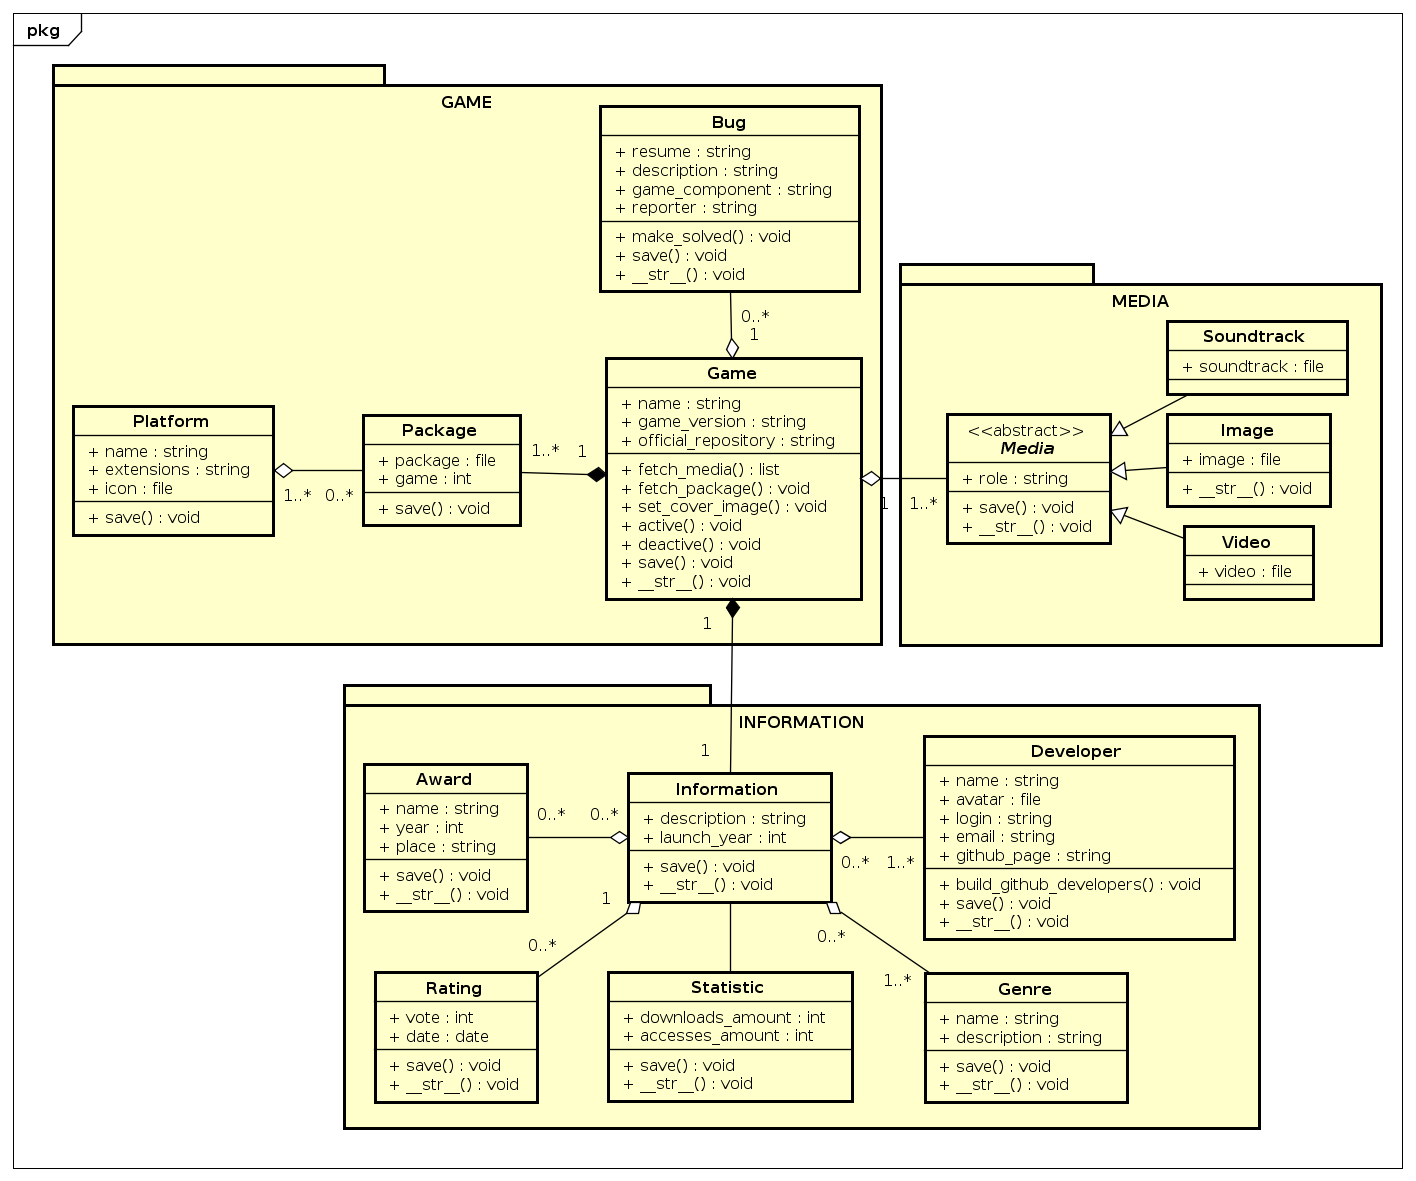
\includegraphics[width=\textwidth,height=\textheight,keepaspectratio]{class_diagram}
\caption{Class Diagram of the Platform \cite{plataforma2017arquitetura}}
\label{fig:class_diagram}
\end{figure}

As the second part of the development started, they had to work on a totally different mindset, with new roles and documents needed. Instead of having managers, the team had now Scrum Master, Product Owner, and the Developing team \cite{cohen2003agile}. A Scrum Master is the responsible for protecting the team, making sure knowledge is being shared and Scrum is being followed \cite{scrumalliance2017}. It's important to notice that this is not equivalent to a traditional manager, that usually only bosses around the team, not caring about the people.

Product Owner is the one who will say the product value, sets the priorities and decides what need be done \cite{agile422017}. They must assure the work meets their expectations without controlling the development team \cite{schwaber2002agile}. The Development Team are the people who will actually do the work, they don't have a manager, they act collectively and decide how they will achieve what has to be done \cite{greer2011agile}.

The second half of the project focused more on the packaging template, with a few corrections and bug reports from FGA students on the platform.


\section{Tools}
\label{sec:tools}

GNU Make and bash were the chosen software for building and packaging. Make is supposed to help developers managing their applications and they can run on several platforms, like Linux, Mac, and Windows. Bash is a popular script tool to manipulate files and folders from the terminal. They are distributed under GNU General Public License version 3 and the minimum required version is 4.0 (for both of them).

The chosen compilers were \texttt{gcc}, for Linux, distributed under GPL3, with at least version 5.0; \texttt{Visual Studio Compiler}, for Windows, shared with a Microsoft community License, version 2017; and \texttt{clang}, for macOS, distributed under BSD License.

For the website development, Django was picked because of the previous knowledge the group had with it. To make the front end of the application, Facebook's React was chosen for the flexibility it gives to the user interface. They are both very scalable, have a big support in the community and are released under the BSD 3-clause license. The versions being used are the last ones at the beginning of the project, namely, 1.11.1, for Django, and 15.5.4, for React.

To develop and test the template, virtual machines running Debian Jessie and CentOS 7 were used. The VMs were powered by VirtualBox 5.2, released under GPL2, that allows easy environment virtualization. It also enables a developer to test in several operating systems, which is required for the nature of this project. The computer hosting the virtual machines and used to has an Intel Core i5-6200U 2.3 GHz processor, 8 GB of RAM and an NVIDIA GeForce 940M graphic processor.

To package on Debian based systems, \texttt{lintian} version 2.5. For Red-Hat systems, \texttt{rpmlintian} version 1.9 was chosen. Both of them are distributed under GPL 2. For Windows, both Wix toolset, version 3.11, distributed under Microsoft Reciprocal License; and Gygwin shell, 2.9.0 and GPL, were used.
